% 2018 May 22 - From Jackson+ (2013) study of HAT-P-7 - "Welsh et al. (2010) discovered ellipsoidal variations in the Kepler Q1 data, with an amplitude of 37.3 ppm. They also estimated that the planet’s phase curve has an amplitude of 31.9 ppm..." - So EVs and planet's phase curve has comparable amplitudes.

\documentclass[manuscript]{aastex}

%% preprint2 produces a double-column, single-spaced document:

%% \documentclass[preprint2]{aastex}

%% Sometimes a paper's abstract is too long to fit on the
%% title page in preprint2 mode. When that is the case,
%% use the longabstract style option.

%% \documentclass[preprint2,longabstract]{aastex}

%% If you want to create your own macros, you can do so
%% using \newcommand. Your macros should appear before
%% the \begin{document} command.
%%
%% If you are submitting to a journal that translates manuscripts
%% into SGML, you need to follow certain guidelines when preparing
%% your macros. See the AASTeX v5.x Author Guide
%% for information.

\newcommand{\kepler}{{\it Kepler}}
\newcommand{\tess}{{\it TESS}}
% \newcommand{\myemail}{skywalker@galaxy.far.far.away}

%% You can insert a short comment on the title page using the command below.

\slugcomment{Submitted to ApJ, Fall 2018}

%% If you wish, you may supply running head information, although
%% this information may be modified by the editorial offices.
%% The left head contains a list of authors,
%% usually a maximum of three (otherwise use et al.).  The right
%% head is a modified title of up to roughly 44 characters.
%% Running heads will not print in the manuscript style.

\shorttitle{Eclipse Variability}
\shortauthors{Jackson, Sandidge, Kreyche, \& Briggs}

%% This is the end of the preamble.  Indicate the beginning of the
%% paper itself with \begin{document}.
\usepackage{hyperref}
\usepackage{graphics,graphicx}

\begin{document}

%% LaTeX will automatically break titles if they run longer than
%% one line. However, you may use \\ to force a line break if
%% you desire.

\title{Searching for Variability in Eclipses in the Kepler Dataset}

%% Use \author, \affil, and the \and command to format
%% author and affiliation information.
%% Note that \email has replaced the old \authoremail command
%% from AASTeX v4.0. You can use \email to mark an email address
%% anywhere in the paper, not just in the front matter.
%% As in the title, use \\ to force line breaks.

\author{Brian Jackson\altaffilmark{1}, Wesley Sandidge, Steven Kreyche, \& Jennifer Briggs}
\affil{Department of Physics, Boise State University\\ 1910 University Drive, Boise ID 83725-1570 USA}

%% Notice that each of these authors has alternate affiliations, which
%% are identified by the \altaffilmark after each name.  Specify alternate
%% affiliation information with \altaffiltext, with one command per each
%% affiliation.

\altaffiltext{1}{bjackson@boisestate.edu}

%% Mark off your abstract in the ``abstract'' environment. In the manuscript
%% style, abstract will output a Received/Accepted line after the
%% title and affiliation information. No date will appear since the author
%% does not have this information. The dates will be filled in by the
%% editorial office after submission.

\begin{abstract}

\end{abstract}

%% Keywords should appear after the \end{abstract} command. The uncommented
%% example has been keyed in ApJ style. See the instructions to authors
%% for the journal to which you are submitting your paper to determine
%% what keyword punctuation is appropriate.

\keywords{}

%% From the front matter, we move on to the body of the paper.
%% In the first two sections, notice the use of the natbib \citep
%% and \citet commands to identify citations.  The citations are
%% tied to the reference list via symbolic KEYs. The KEY corresponds
%% to the KEY in the \bibitem in the reference list below. We have
%% chosen the first three characters of the first author's name plus
%% the last two numeral of the year of publication as our KEY for
%% each reference.


%% Authors who wish to have the most important objects in their paper
%% linked in the electronic edition to a data center may do so by tagging
%% their objects with \objectname{} or \object{}.  Each macro takes the
%% object name as its required argument. The optional, square-bracket 
%% argument should be used in cases where the data center identification
%% differs from what is to be printed in the paper.  The text appearing 
%% in curly braces is what will appear in print in the published paper. 
%% If the object name is recognized by the data centers, it will be linked
%% in the electronic edition to the object data available at the data centers  
%%
%% Note that for sources with brackets in their names, e.g. [WEG2004] 14h-090,
%% the brackets must be escaped with backslashes when used in the first
%% square-bracket argument, for instance, \object[\[WEG2004\] 14h-090]{90}).
%%  Otherwise, LaTeX will issue an error. 


\section{Introduction}

\section{Data Analysis}
\subsection{Data Conditioning}
For each system's light curve, we applied the following steps to condition each quarter's the long-cadence (i.e., 30-min integration times) data:
\begin{enumerate}
\item We subtracted the median value from each quarter's PDCSAP\_FLUX time-series, before dividing through by that same median value.
\item We next applied a median boxcar filter with a window size equal to an integer number $n$ of orbital periods for the target -- for each system, we considered $n$ from one up to five, choosing the value that maximizes the eclipse signal when we fold together all the available data on the best-fit orbital period from previous analyses. To mitigate edge-effect distortions, we extended the time-series beyond both ends out a full window length by reflecting the original time-series across its boundary.
\item Finally, we stitched each quarter's conditioned data into one long time-series and subtracted the average value of the planet's eclipse (i.e., we zeroed out the eclipse) because, in principle, only the star's light registers during that phase so it sets the baseline against which to measure the photometric variations. Since our phase curve model allows for an arbitrary offset value, zeroing out the eclipse has no physical significance.
\end{enumerate}
Figure \ref{fig:Analysis_of_Kepler76b_data} illustrates a portion of the raw and conditioned time-series for Kepler-76 b. 

\subsection{Model}

After applying the above conditioning procedure, we folded together all available data on the transit ephemeris from a previous study (each planet's section below gives the corresponding references) and, using a Markov-Chain Monte-Carlo analysis \citep{}, we fit the folded transit, eclipse, and out-of-transit variations using the following model:
\begin{equation}
    \Delta F = T\left(\phi\right) + A_{\rm beam} \sin\left(2\pi\phi\right) - A_{\rm ellip} \cos\left( 2 \times 2\pi\phi \right) + E \bigg( F_{\rm 0} - A_{\rm planet} \cos\left[ 2\pi\left( \phi - \Delta \phi \right) \right] \bigg), \label{eqn:photometric_model}
\end{equation}
where $\Delta F$ is the normalized photometric variation, $\phi$ the orbital phase (0 at mid-transit, 0.5 at mid-eclipse), and $T$ the transit signal (modeled using \citealt{2002ApJ...580L.171M} as implemented in PyAstronomy\footnote{https://github.com/sczesla/PyAstronomy}). In the equation, the second term represents the beaming effect, with $A_{\rm beam}$ as its amplitude, and the third term represents the ellipsoidal variations, with $A_{\rm ellip}$ as its amplitude. The very last term models the planet's phase curve: $F_{\rm 0} - A_{\rm planet}$ represents the minimum in the planet's photometric contribution at $\phi - \Delta \phi = 0$, and $F_{\rm 0} + A_{\rm planet}$ the peak in the phase curve at $\phi - \Delta \phi = 0.5$, with $\Delta \phi$ allowing for a phase offset, which has been reported for some planets (refs). $E$ represents the planet's eclipse signal and takes on whatever fraction of the planet's disk remains unocculted (unity outside of eclipse and zero at mid-eclipse for a completely occulted planet).

the Levenburg-Marquardt to fit a standard transit light curve \citep{2002ApJ...580L.171M} appropriately convolved over the to the mid-transit times for all the transits in each dataset and confirmed they conformed to a linear ephemeris, finding no evidence for transit-timing variations. (Below we report new ephemerides slightly updated relative to previous analyses for each object.) 

\begin{figure}
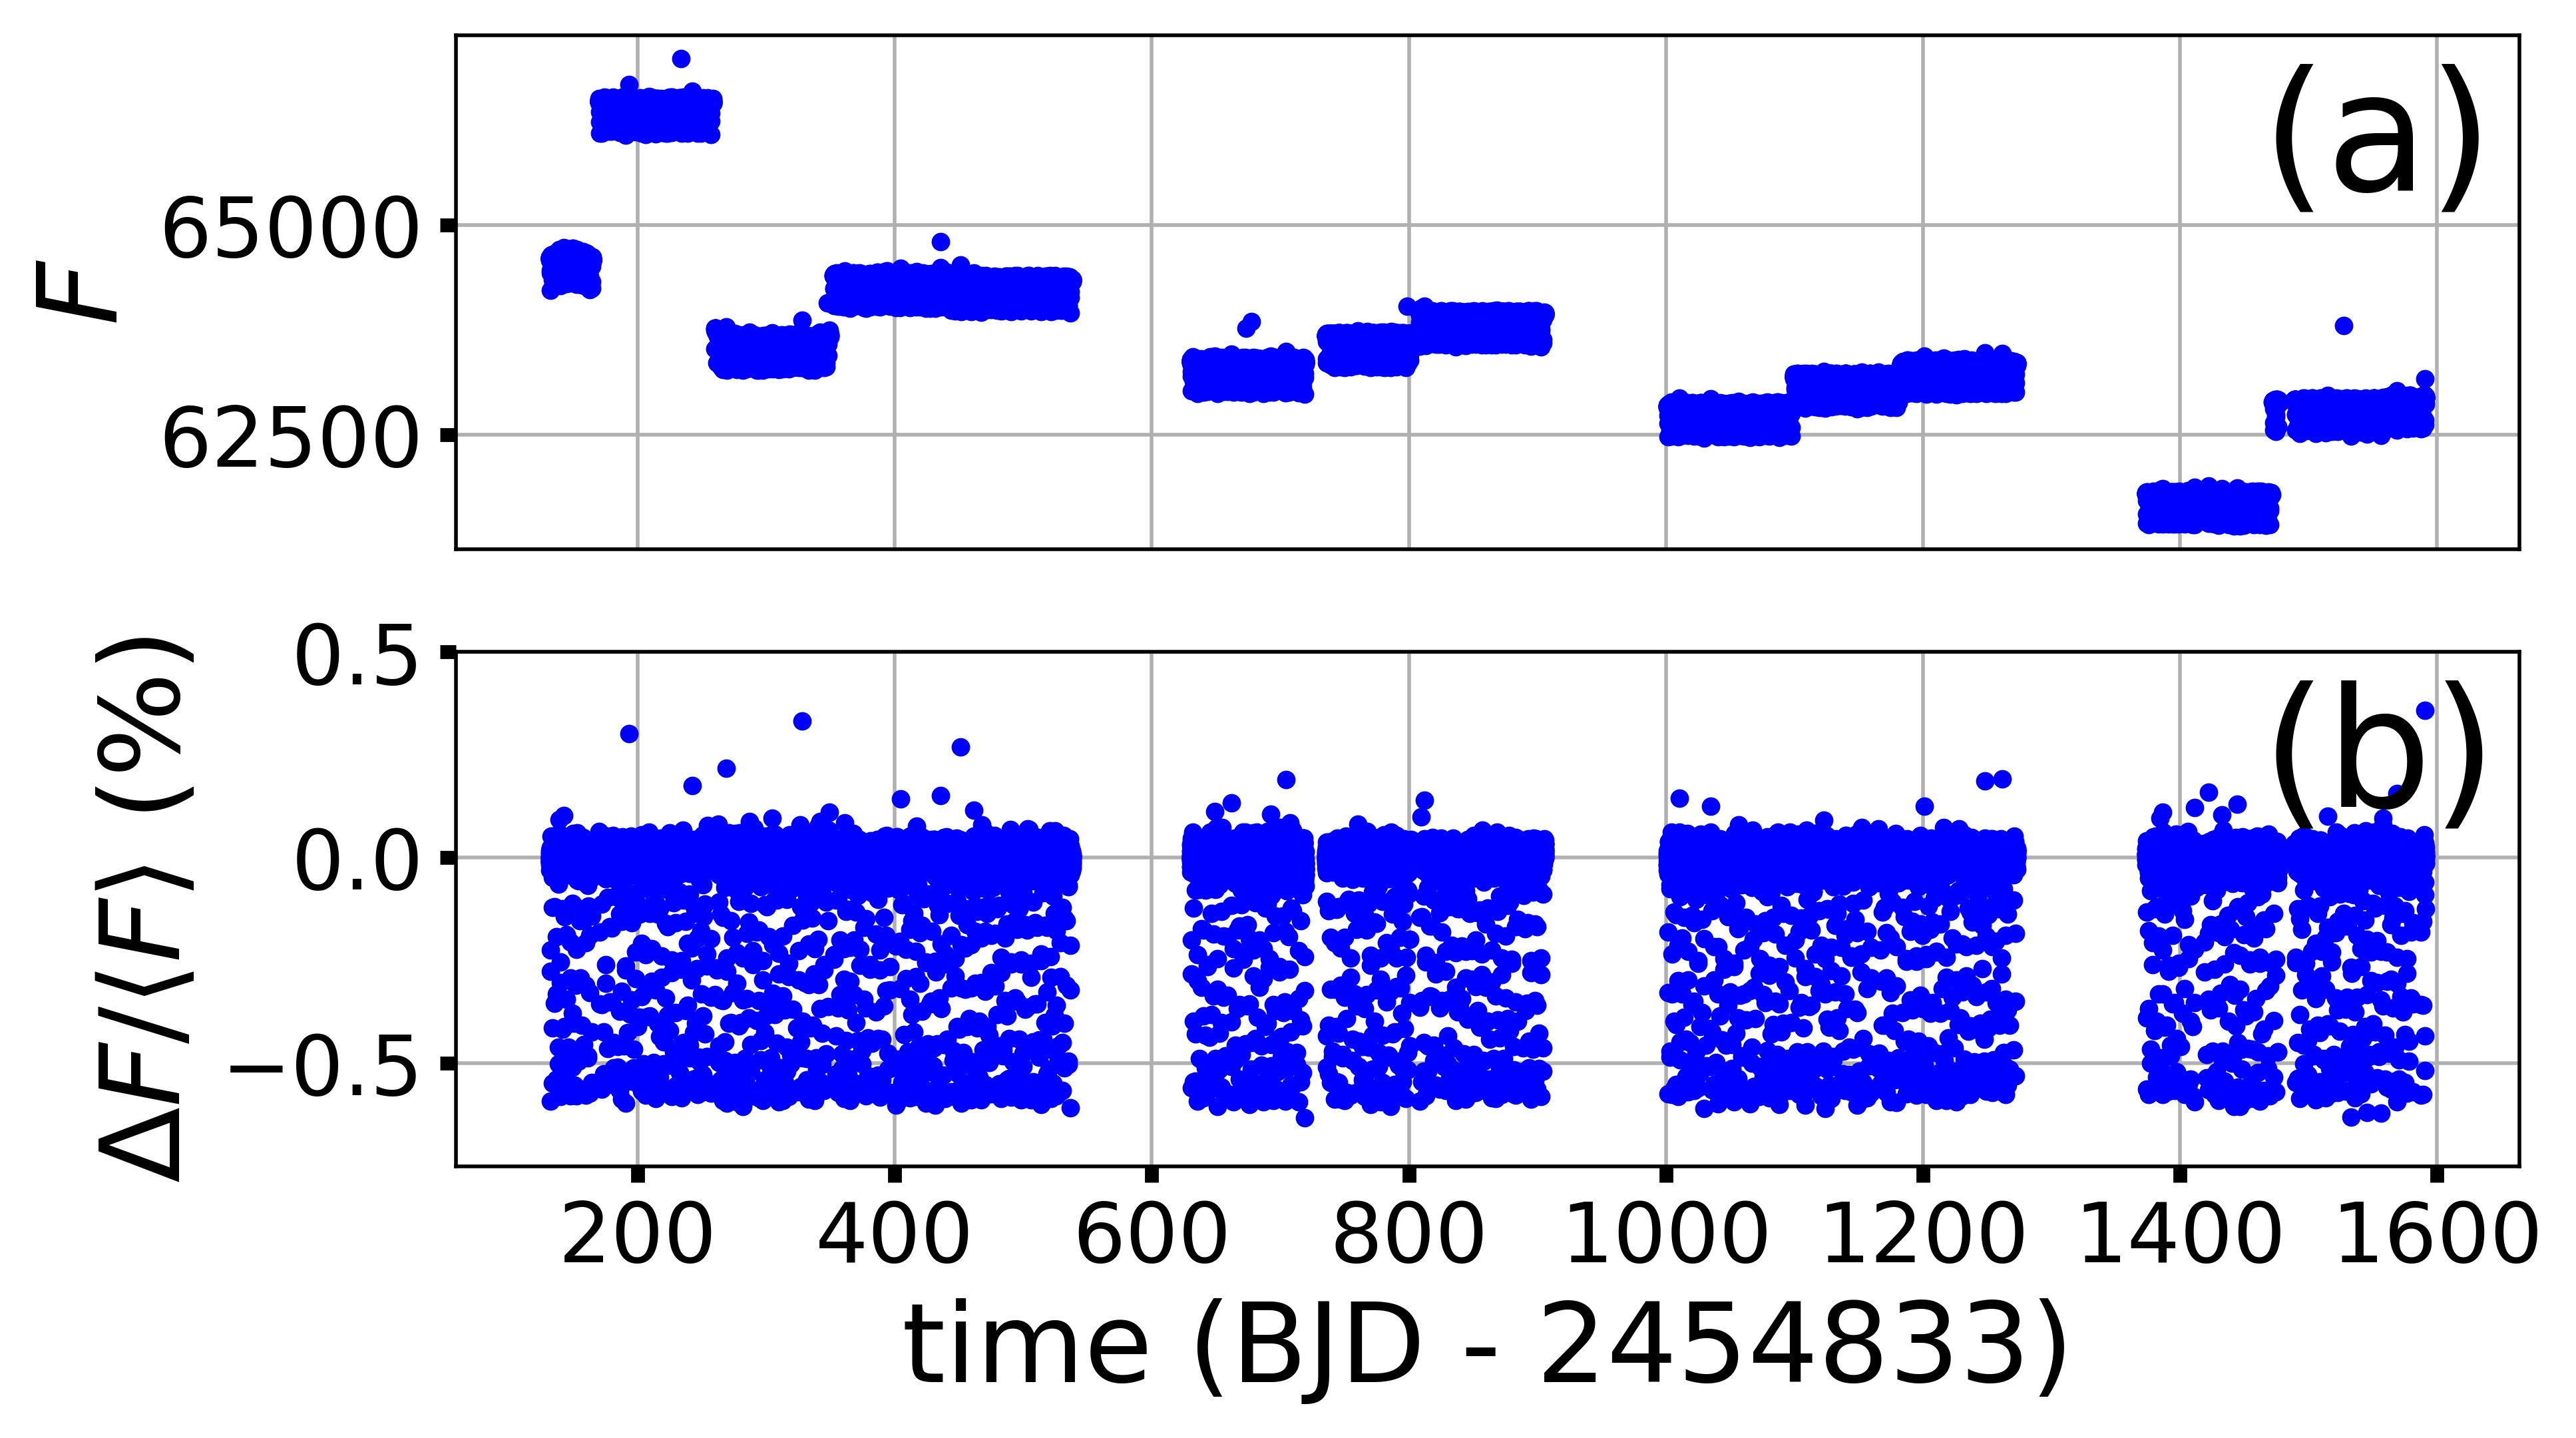
\includegraphics[width=\textwidth]{Analysis_of_Kepler76b_data.jpg}
\caption{The quarter-by-quarter Raw (a) and conditioned (b - in \%) PDCSAP\_FLUX. Time along the x-axis is shown in the \kepler\ mission's barycentric Julian date minus 2454833 (midnight on 2009 January 1), and the y-axis shows variations in flux. \label{fig:Analysis_of_Kepler76b_data}}
\end{figure}

\section{Results}

\section{Discussion and Conclusions}
Figure \ref{fig:eclipse_estimates} shows estimates of signal-to-noise ratios (SNR) expected for secondary eclipses observed by \tess\ based on the synthetic population of planets in the \tess\ yield calculations from \citet{2018arXiv180405050B}. For each synthetic planet from that study, we estimated the eclipse depth $\Delta$ for the case that the planet reflects all of the light it receives from the star (shown in blue) and for the case that the planet emits (and absorbs) light as a perfect blackbody (shown in orange). For the former case, the eclipse depth is given as $\frac{1}{4} \left( \frac{R_{\rm p}}{a} \right)^2$, where $R_{\rm p}$ is the planetary radius and $a$ is the orbital semi-major axis. We then estimated the corresponding SNR by multiplying the transit SNRs given for each planet by planet-star radius ratio squared and then by $\Delta_{\rm reflected}$. For the latter case, we used the stellar insolation given for each planet and assumed dayside thermal equilibrium with zero albedo for each planet to estimate a brightness temperature and convolved the resulting blackbody curve against the \tess\ spectral response function\footnote{https://tessgi.github.io/TessGiWebsite/the-tess-space-telescope.html}. We combined the insolation and planet's orbital distance to estimate the stellar effective temperature and, likewise, convolved the corresponding blackbody curve against the response function. Finally, we divided the planet's convolved brightness by the star's and used the re-scaled transit SNR to calculate the SNR for the thermally emitted eclipse. Figure \ref{fig:eclipse_estimates} only shows those SNR-values $> 3$, among which the vast majority (54 of 62 total) have $R_{\rm p} \geq 10\ R_{\rm Earth}$.

The synthetic population from \citet{2018arXiv180405050B} included 4,553 planets, and Figure \ref{fig:eclipse_estimates} suggests only about 1\% of these may have secondary eclipses detectable for \tess. However, among those, our calculation suggests that the eclipse signals will be considerably more sensitive to emitted than reflected light, in contrast to the eclipses observed by \kepler\ (ref), which owes largely to the fact that the \tess\ spectral response function is more sensitive at longer wavelengths than that of \kepler. Presumably, this different sensitivity also means detectable \tess\ eclipses will probe atmospheric thermal structures more than \kepler\ eclipses could.

% XXX and something about eclipse variability XXX

% How detectable will be the ellipsoidal variations?

\acknowledgments

%% To help institutions obtain information on the effectiveness of their
%% telescopes, the AAS Journals has created a group of keywords for telescope
%% facilities. A common set of keywords will make these types of searches
%% significantly easier and more accurate. In addition, they will also be
%% useful in linking papers together which utilize the same telescopes
%% within the framework of the National Virtual Observatory.
%% See the AASTeX Web site at http://aastex.aas.org/
%% for information on obtaining the facility keywords.

%% After the acknowledgments section, use the following syntax and the
%% \facility{} macro to list the keywords of facilities used in the research
%% for the paper.  Each keyword will be checked against the master list during
%% copy editing.  Individual instruments or configurations can be provided 
%% in parentheses, after the keyword, but they will not be verified.

{\it Facilities:} \facility{Kepler}.
\software{numpy, astropy, statsmodels, scipy, lightkurve, BEER\_curve, dill, PyAstronomy, emcee}

\bibliographystyle{aasjournal}
\bibliography{bibliography}

\begin{figure}

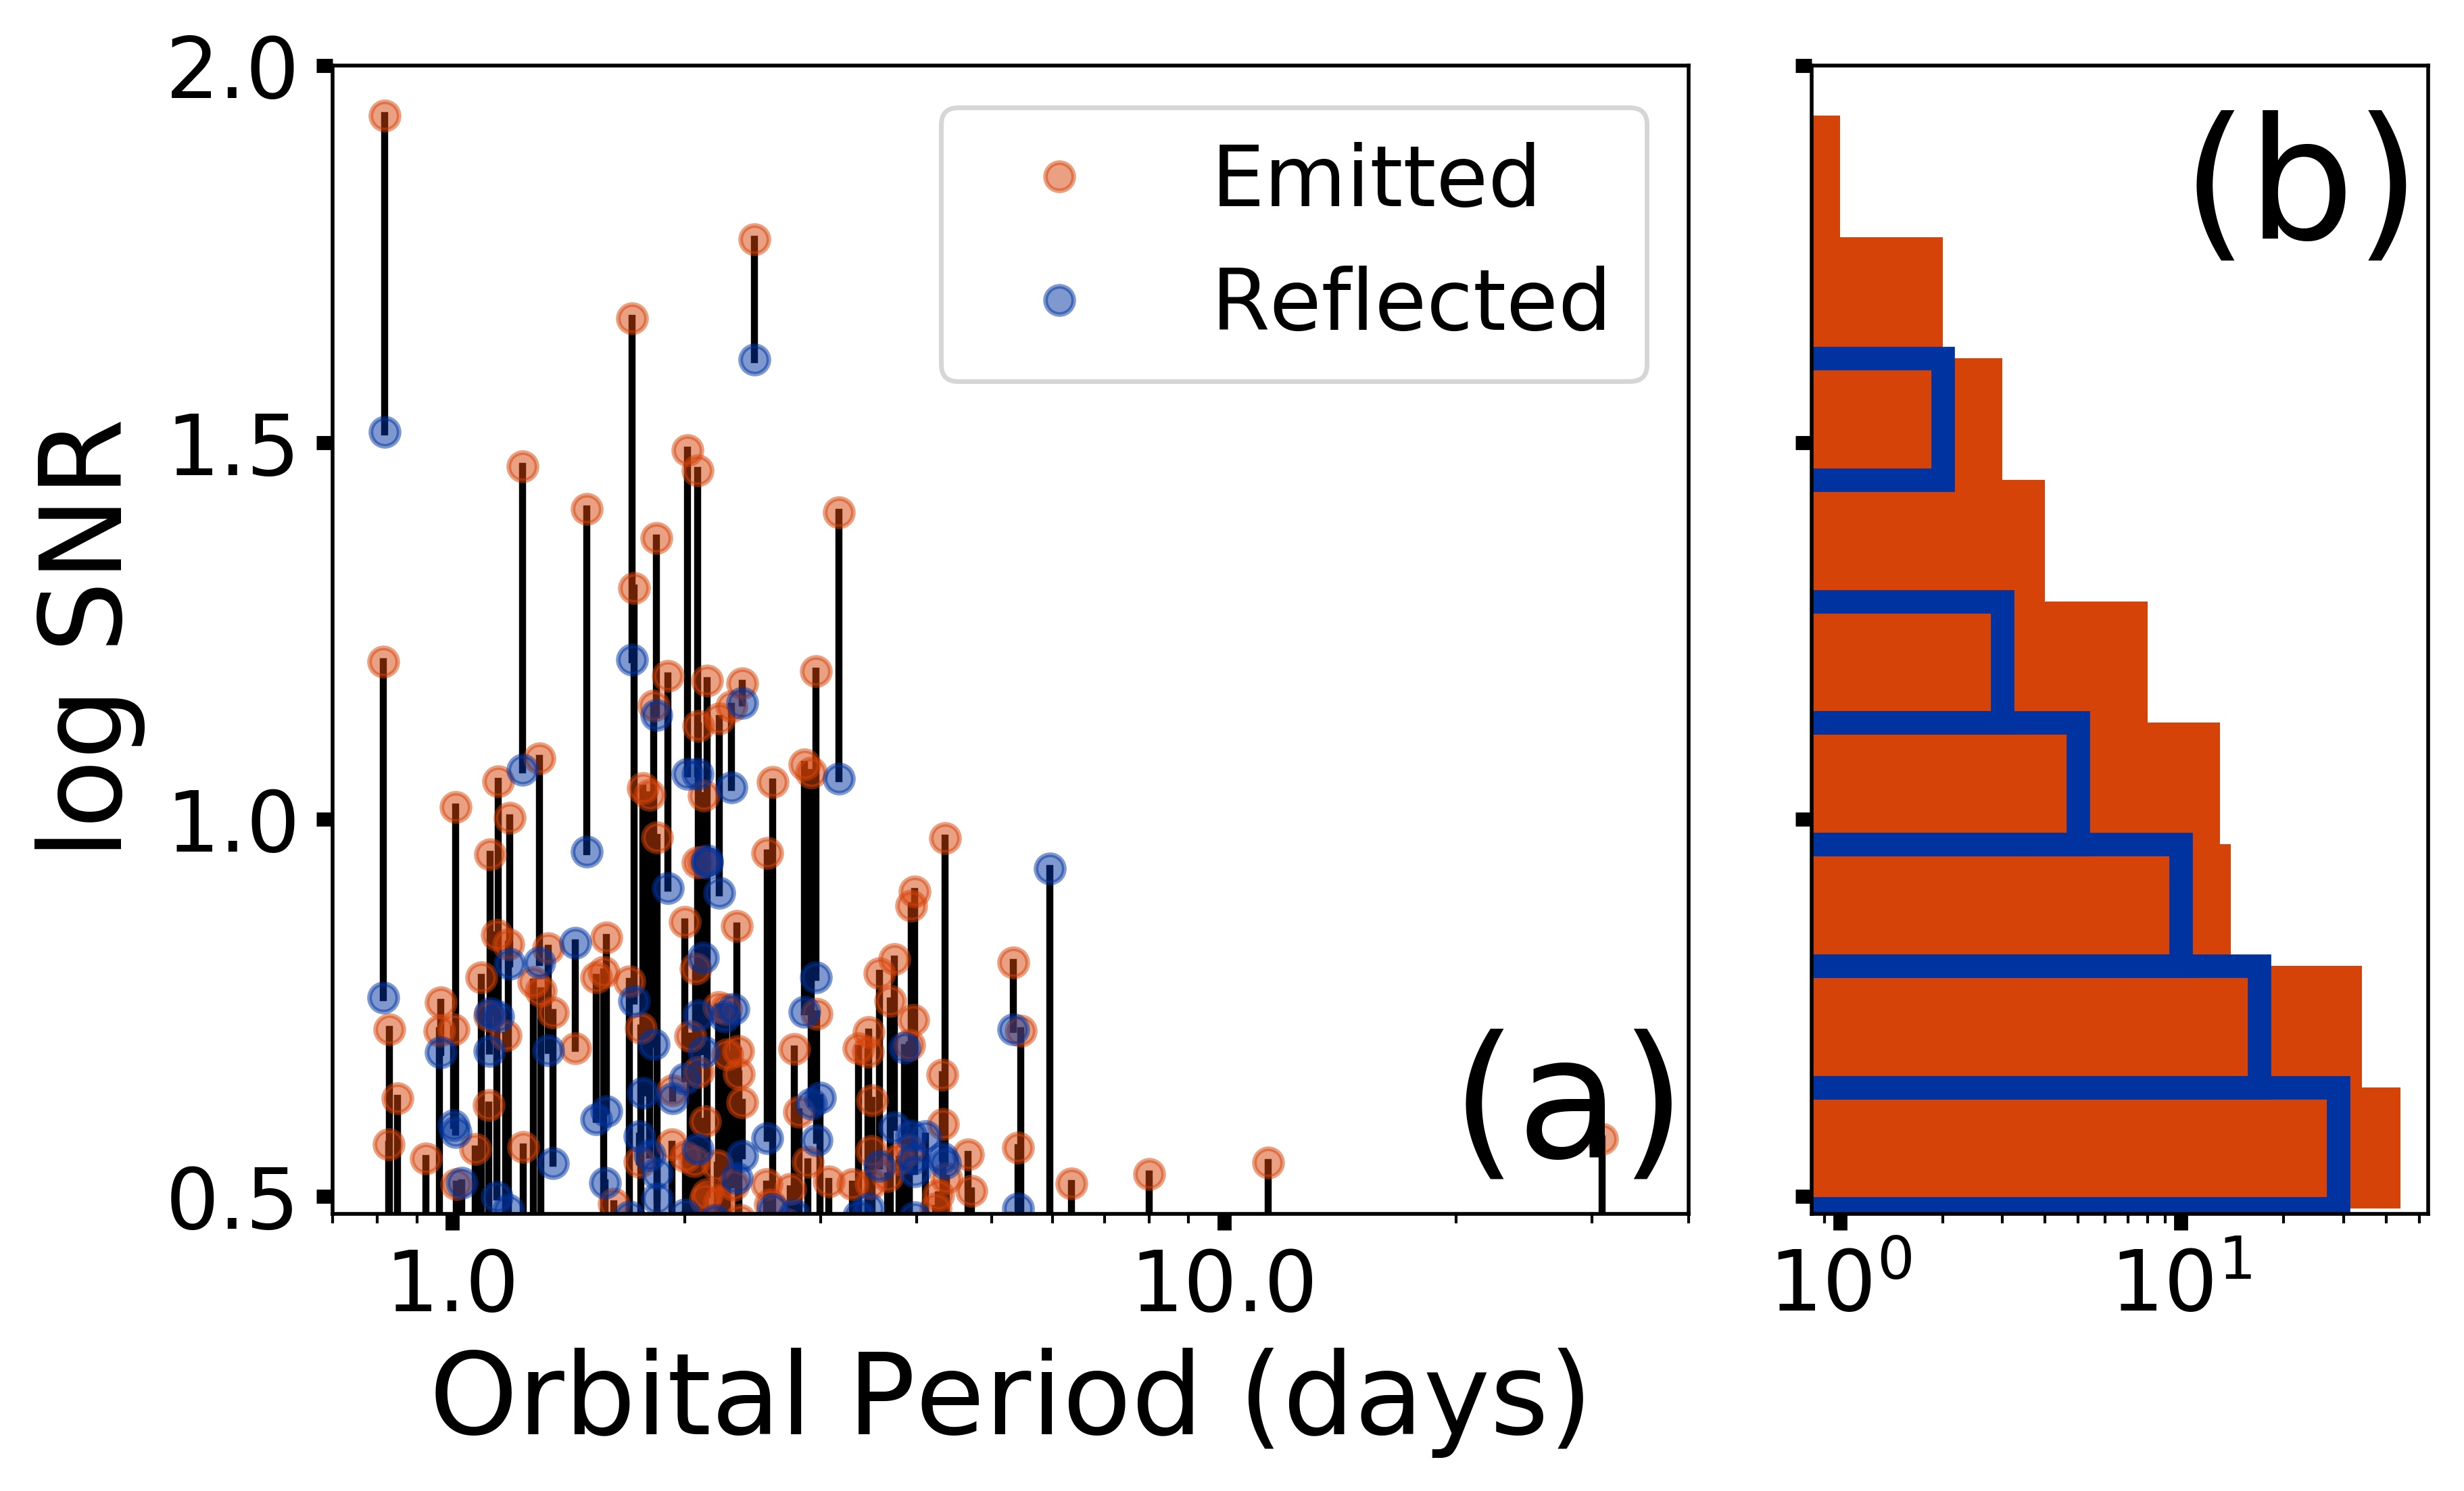
\includegraphics[width=\textwidth]{eclipse_estimates.jpg}
\caption{The $\log$ of the signal-to-noise ratio $SNR$ for planetary secondary eclipses for a population of synthetic planets from the \tess\ mission yield study of \citet{2018arXiv180405050B}. The blue dots in (a)  show eclipses for perfectly reflecting planets, while the orange dots show eclipses for perfect blackbody planets, with black lines connecting the two eclipses for each planet. Panel (b) shows a histogram of SNR-values. \label{fig:eclipse_estimates}}

\end{figure}

\end{document}

%%
%% End of file `sample.tex'.